\section{Performance Evaluation}

Two platforms were for performance evaluation of our novel \textit{PackDrop} scheduler:
i) A tightly coupled \textbf{Supercomputer}with $24$ (in $2$ NUMA nodes) PEs per thin node, using a fast Infiniband interconnection supported by Intel's Parallel Studio XE implementation of \texttt{MPI} (v2017.4).
ii) A traditional computational \textbf{Cluster} with $4$ PEs per node, using a Gigabit Ethernet interconnection.
Details of both platforms are available on Table~\ref{tab:ptinfo}.

\begin{table}[ht]
    \centering
	\begin{tabular}{c|c|c}
	Node Info.	 		& Supercomputer 		& Cluster \\ \hline
        CPUs	   			& $2\times12$ 			& $4$ \\
        Intel Xeon			& E5-2695v2 			& X3440\\
        CPU Freq.  			& $2.4$GHz   			& $2.53$GHz\\
        RAM        			& $64$GB			& $16$GB\\
        Network 			& Infiniband FDR 		& Gigabit Ethernet\\
        OS      			& RedHat Linux 6.4 		& Ubuntu 14.04\\
        \texttt{GCC}			& $5.3.1$			& $5.4.0$\\
        \texttt{Charm++} 		& $6.8.1$ 			& $6.8.1$\\
        \texttt{MPI}			& $3.1.0$			& -\\
        \texttt{GCC} Flags		& \texttt{-std=c++11 -O3} 	& \texttt{-std=c++11 -O3} \\
	\end{tabular}
    \caption{Platform Information of each Node from Supercomputer and Cluster evaluations. }
    \label{tab:ptinfo}
\end{table}



\subsubsection*{Metrics}

\subsection{Evaluation on Supercomputer}

\subsection{Evaluation on Cluster}

All experiments ran on cluster were compiled with \texttt{Charm++} using the \texttt{--with-production} option, combined with the specifications detailed on Table~\ref{tab:ptinfo}.
$32$ equal compute nodes were used, with a total of \textbf{128 PEs}.
In addition to previously mentioned schedulers, \textit{Dummy} was added\textbf{} as the representative of a situation with no remap of tasks.

\subsubsection*{Evaluation with Synthetic Load}

\textbf{LB Test} experiments had a total of $18990$ \textit{tasks}, executed over $150$ iterations, performing load balance every $40$ iterations.
\textit{Task} loads vary from $30$ms to $9000$ms, which provides reasonable imbalance of load, causing global rescheduling to be useful in this case.
Ring, two-dimensional (2D) and 3D mesh communication topologies were used to provide different levels of migration impact and communication cost.

\begin{table}[t]
	\centering
	\begin{tabular}{l | c | c | c}
    	Scheduler & Time (Ring) & Time (2D) & Time (3D) \\ \hline
        Distributed & $47.49298$s & $48.64839$s & $49.05481$s \\
        Greedy & $46.54101$s & $49.56052$s & $51.06850$s \\
        Dummy & $52.43016$s & $53.17254$s & $53.94068$s \\
        PackDrop & $46.81598$s & $47.37120$s & $47.97426$s \\
        Refine & $45.49095$s & $46.29277$s & $47.21924$s \\		
	\end{tabular}
    \caption{LB Test mean application time on the cluster execution.}
    \label{tab:lbtest:apptime}
\end{table}

\begin{figure}
	\centering
    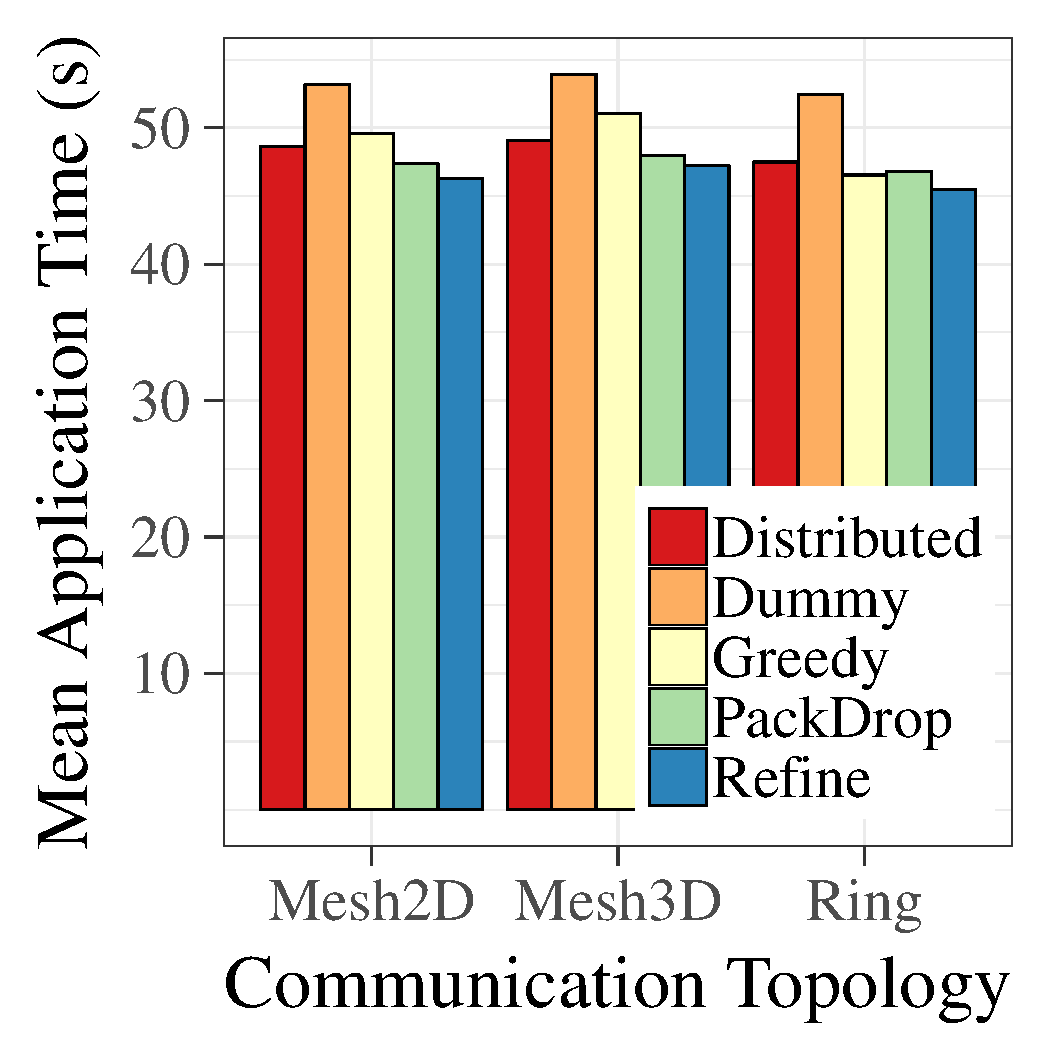
\includegraphics[width=0.4\textwidth]{images/apptime_lbtest_g5k.pdf}
    \caption{LB Test cluster execution results.}
    \label{fig:eval:g5k:lbtest:apptime}
\end{figure}


Each configuration of the benchmark was executed $15$ times, with results depicted on Figure~\ref{fig:eval:g5k:lbtest:apptime} and Table~\ref{tab:lbtest:apptime}.
Results for \textit{Greedy} show how different communication topologies affect the scheduling performance.
Since \textit{Greedy} migrates many \textit{tasks}, the more they communicate, the more migrations impact the application time.

The increased in communication cost can be verified among all scheduling strategies, but in none as much as in \textit{Greedy}.
Our novel approach, \textit{PackDrop} has outperformed the closest approach, \textit{Distributed} in the \textit{LB Test} case of this scale.
However, since the platform is not large enough to present the potential gains of decentralized strategies, \textit{Refine}, with a reduced migration count approach, still outperforms any other scheduler in this benchmark.

\subsubsection*{Evaluation with Molecular Dynamics}

\textbf{LeanMD} experiments generated a $10\times15\times10$ space, with a total of $57000$ \textit{tasks}.
Each execution ran $100$ iterations, with a first rescheduling step at the $10$th iteration. 
Load balancing periods of every $10$ and every $30$ iterations were used, providing different impacts of rescheduling on the application.

Each configuration of LeanMD was executed $10$ times, making a total of $1000$ steps per configuration. 

\todo[inline]{Do experiments with MD again on cluster. Try 3 different LB freq. since Refine seems to produce a more stable mapping of the system.}

\begin{figure}
	\centering
    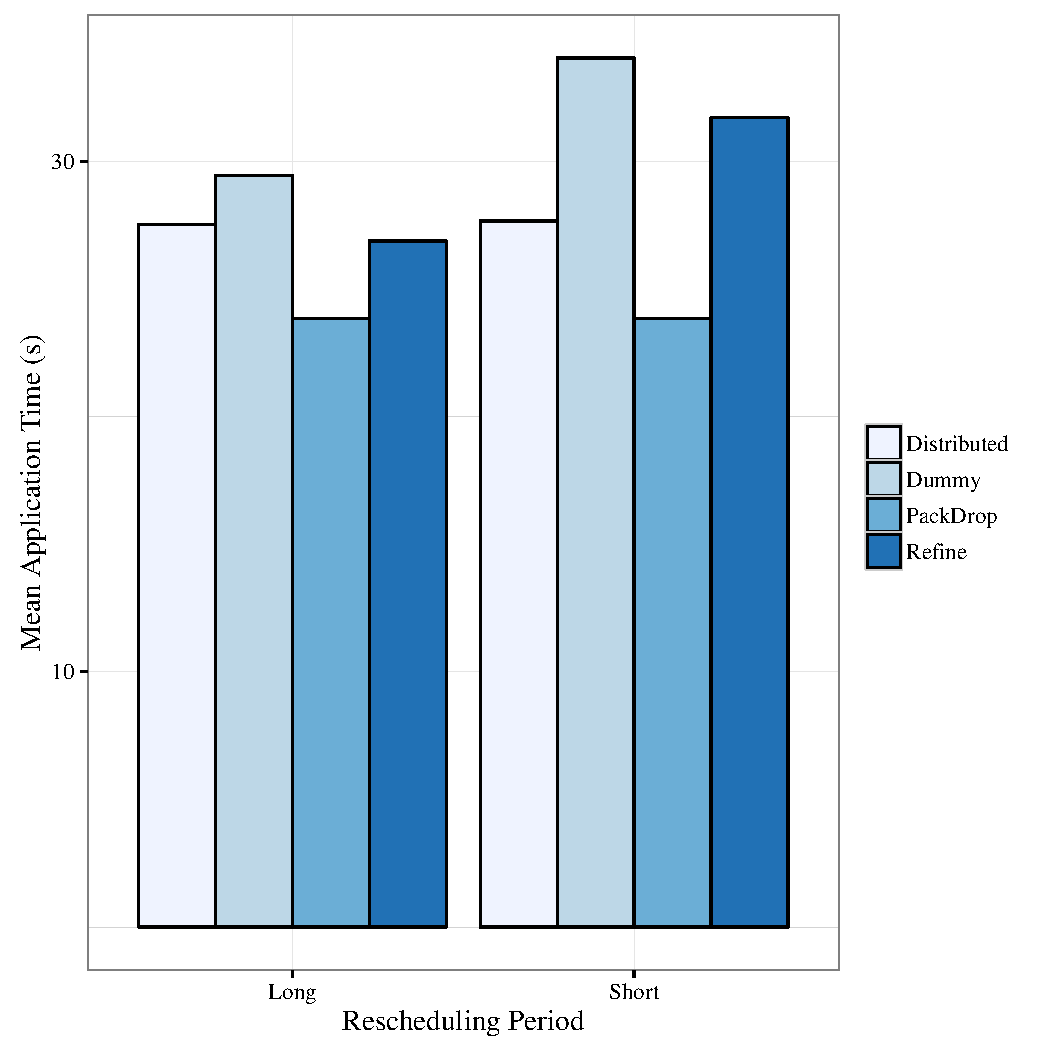
\includegraphics[width=0.2\textwidth]{images/apptime_leanmd_g5k.pdf}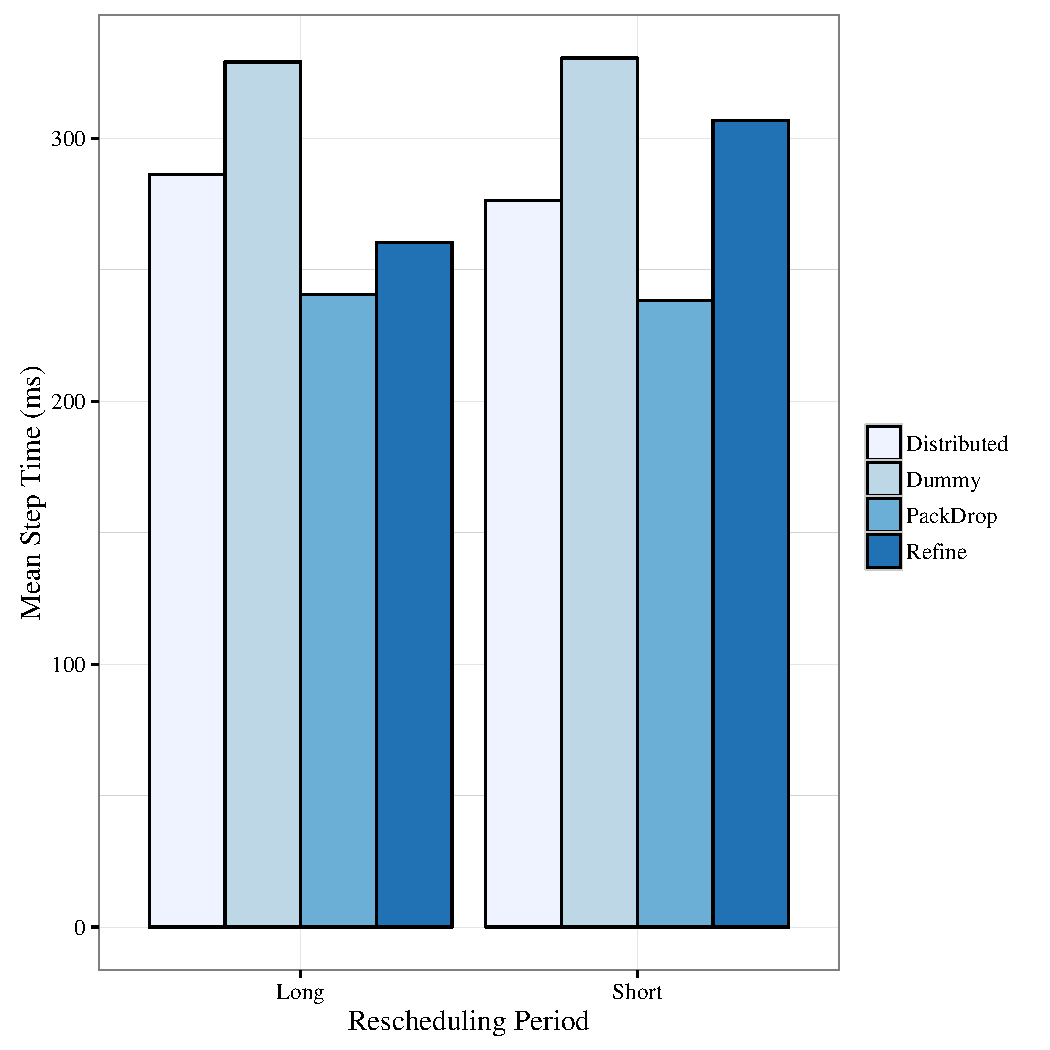
\includegraphics[width=0.2\textwidth]{images/steptime_leanmd_g5k.pdf}
    \caption{LeanMD cluster execution results.}
    \label{fig:eval:g5k:leanmd:time}
\end{figure}

\subsection{Scalability}